\documentclass[unicode, notheorems, handout]{beamer}

\usetheme[numbers,totalnumbers,compress, nologo]{Statmod}
\usefonttheme[onlymath]{serif}
\setbeamertemplate{navigation symbols}{}

\mode<handout> {
	\usepackage{pgfpages}
    %\setbeameroption{show notes}
	%\pgfpagesuselayout{2 on 1}[a4paper, border shrink=5mm]
	\setbeamercolor{note page}{bg=white}
	\setbeamercolor{note title}{bg=gray!10}
	\setbeamercolor{note date}{fg=gray!10}
}

\usepackage[T2A]{fontenc}
\usepackage[utf8x]{inputenc}
\usepackage[russian]{babel}
\usepackage{tikz}
\usepackage{ragged2e}
\usepackage{subcaption}
\usepackage{mathtools}
\usepackage{array}
\usepackage{pifont}
\usepackage{xcolor}

\definecolor{darkblue}{rgb}{0,0,0.5}

\newtheorem{corollary}{Следствие}
\newtheorem{proposition}{Предложение}
\newtheorem{definition}{Определение}


\title[Обучение без учителя. Кластеризация]{Обучение без учителя. Кластеризация}


\institute[Санкт-Петербургский Государственный Университет]{%
	\small
	Санкт-Петербургский государственный университет\\
	Кафедра статистического моделирования\\
    Семинар <<Статистическое и машинное обучение>>
}

\date[Октябрь 2025]{Санкт-Петербург, 2025}

\begin{document}

\begin{frame}
	\titlepage
\end{frame}

\begin{frame}{Обучение без учителя}

\textbf{Обучение без учителя (unsupervised learning)} --- раздел машинного обучения, изучающий класс задач обработки данных, в которых известны только описания множества объектов (признаки объектов) из обучающей выборки, и требуется обнаружить внутренние зависимости, существующие между объектами. В отличие от обучения с учителем, правильные <<ответы>> или <<метки>> для объектов неизвестны.

\end{frame}

\begin{frame}{Задачи обучения без учителя}


    \begin{itemize}
        \item \textbf{Кластеризация.}  Разделение объектов на группы (кластеры) на основании их сходства. 
        \vspace{1ex}

        
        \item \textbf{Поиск ассоциативных правил.} Выявление связей между объектами.  Цель --- найти закономерности вида <<Если встречается $A$, то с высокой вероятностью встречается и $B$>>, где $A,B$ --- некоторые не пересекающиеся наборы признаков.
        \vspace{1ex}

        
        \item \textbf{Понижение размерности.} Уменьшение количества признаков при сохранении максимально возможной информации из исходных данных.
        \vspace{1ex}
        
        \item \textbf{Заполнение пропусков.} Восстановление отсутствующих данных на основе закономерностей, найденных в имеющихся данных.
    \end{itemize}
\end{frame}

\begin{frame}{Постановка задачи кластеризации}
    
  \textbf{Дано:}
   \vspace{0.5ex}
   
 $\pmb{X} $ ---  пространство объектов;
 \vspace{0.5ex}
    
$\pmb{X}^n = \{\pmb{x}_1, \dots, \pmb{x}_n\}$ --- выборка из $\pmb{X}$, где $\pmb{x}_i$ --- $i$-й объект;
\vspace{0.5ex}
     
$\rho: \pmb{X} \times \pmb{X} \to [0, \infty)$ --- функция расстояния между объектами.
\vspace{2ex}

\textbf{Найти:}
 \vspace{0.5ex}
  
 $Y$ ---  множество кластеров;
 \vspace{0.5ex}
 
 $a: \pmb{X} \rightarrow Y$ ---  алгоритм кластеризации. 
  \vspace{0.8ex}


  Причем $Y$ и $a$ такие, что 

  \begin{itemize}
      \item каждый кластер состоит из близких объектов (относительно~$\rho$);
      \item объекты разных кластеров существенно различаются.
  \end{itemize}
\end{frame}

\begin{frame}{Некорректность задачи кластеризации}
    Решение задачи кластеризации неоднозначно:
  \vspace{1ex}
  
    \begin{itemize}
        \item точной постановки задачи кластеризации нет;
        \vspace{0.5ex}
        
        \item существует много критериев качества кластеризации;
          \vspace{0.5ex}
          
        \item число кластеров, как правило, неизвестно заранее;
          \vspace{0.5ex}
          
        \item результат кластеризации сильно зависит от метрики $\rho$, выбор которой также не однозначен.
    \end{itemize}
\end{frame}

\begin{frame}{Типы кластерных структур}
    \begin{figure}[h]
      \centering
    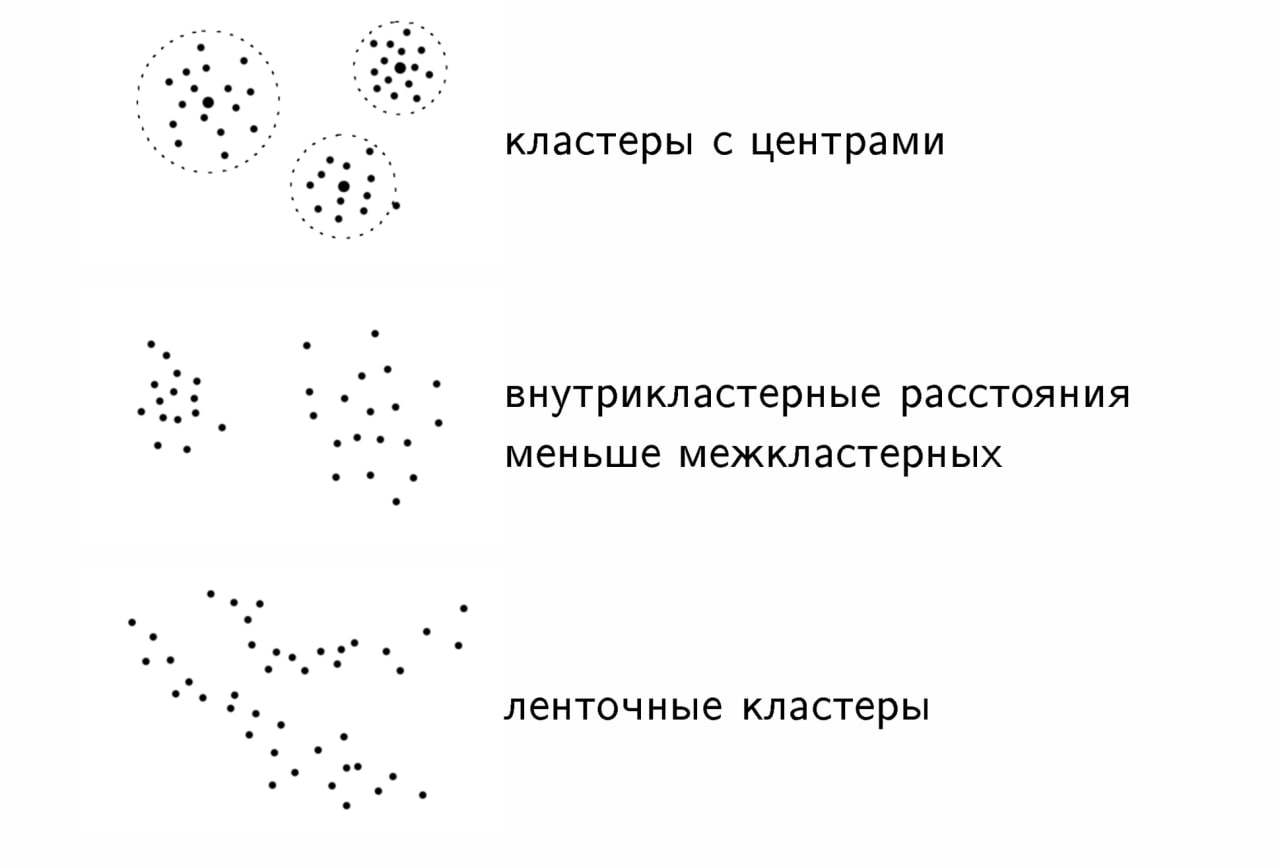
\includegraphics[width=0.99\textwidth]{clust1.jpg} 
    \end{figure}
\end{frame}

\begin{frame}{Типы кластерных структур}
    \begin{figure}[h]
      \centering
    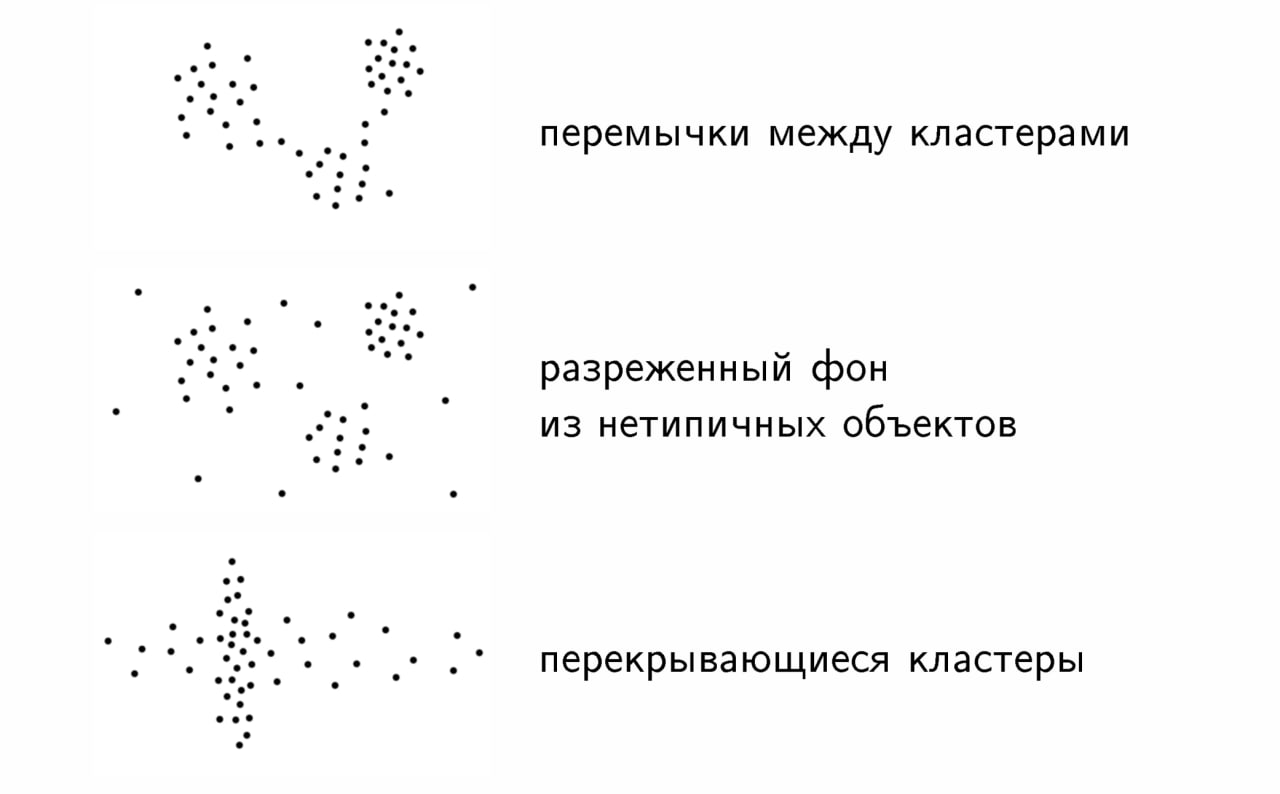
\includegraphics[width=0.99\textwidth]{clust2.jpg} 
    \end{figure}
\end{frame}

\begin{frame}{Типы кластерных структур}

\begin{figure}[h]
      \centering
    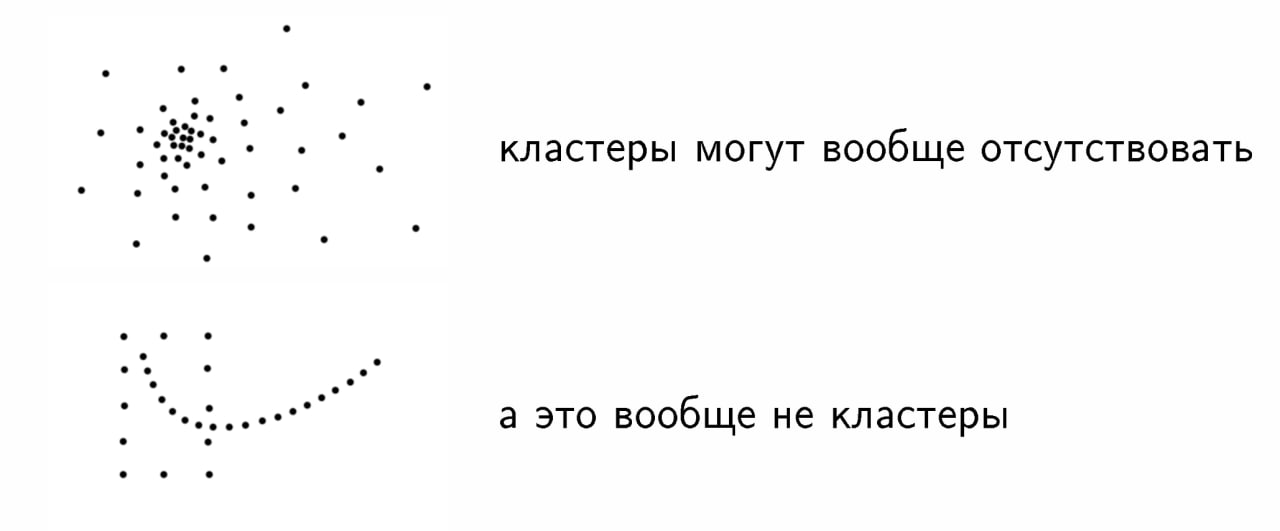
\includegraphics[width=0.9\textwidth]{clust3.jpg} 
    \end{figure}
    
\begin{itemize}
    \item Каждый метод кластеризации имеет свои ограничения и выделяет кластеры лишь некоторых типов. 
    \item Понятие <<тип кластерной структуры>> зависит от метода и также не имеет формального определения. 
\end{itemize}
    
\end{frame}

\begin{frame}{Классификация алгоритмов}
В большинстве источников выделяют пять групп алгоритмов:
\begin{itemize}
    \item \textbf{Основанные на центроидах (centroid based):}
k-means, k-modes, k-medoids, \textbf{\textcolor{darkblue}{Meanshift}}, Affinity Propagation

\item \textbf{Иерархические (hierarchical):} агломеративные (Ward/single/average/complete linkage), BIRCH, на основе теории графов (выделение связных компонент и минимальное остовное дерево), Spectral Clustering

\item \textbf{Основанные на плотности (density based):} \textbf{\textcolor{darkblue}{DBSCAN}}, \textbf{\textcolor{darkblue}{HDBSCAN}}, \textbf{\textcolor{darkblue}{OPTICS}}

\item \textbf{Сеточные (grid based):} STING, Wave cluster, \textbf{\textcolor{darkblue}{CLIQUE}}, OptiGrid, MAFIA

\item \textbf{Основанные на модели данных (model based):} \textbf{\textcolor{darkblue}{Expectation Maximization (EM)}}, COBWEB 
\end{itemize}
\end{frame}


\begin{frame}{EM-алгоритм для model-based подхода}

\textbf{Model-based clustering} --- подход с четко поставленной задачей: предполагаем какую-то статистическую модель данных и в ней находим параметры.
\vspace{0.5ex}

Выборка $\pmb{X}^n$ --- случайна, независима и взята из смеси распределений, плотность которой в точке $\pmb{x} \in \pmb{X}^n$ представима в  виде:

$$p(\pmb{x}) = \sum\limits_{j = 1}^k w_j p_j(\pmb{x}; \pmb{\theta}_j),\; \text{при этом }$$
\vspace{-2ex}

\begin{itemize}
    \item $\sum\limits_{j = 1}^k w_j = 1$, $w_j \geq 0$ --- априорные вероятности кластеров.
    \vspace{1ex}
    
    \item  $p_j(\pmb{x}; \pmb{\theta}_j)$ --- плотность распределения $j$-го кластера с параметрами $\pmb{\theta}_j$.
\end{itemize}
\end{frame}


\begin{frame}{EM-алгоритм для model-based подхода}

Предполагается, зная число кластеров $k$ и вид плотностей $p_j$, оценить параметры $w_j, \pmb{\theta}_j$, максимизируя логарифм функции правдоподобия

$$ \ln L(\{\pmb{x}_i\}; \{w_j\}; \{\pmb{\theta}_j\}) = \sum_{i=1}^n \ln \sum_{j=1}^k w_j p_j(\pmb{x}_i; \pmb{\theta}_j) \rightarrow \max_{\{w_j\}, \{\pmb{\theta}_j\}}.$$

Для решения данной задачи применяется \textbf{ЕМ-алгоритм}.
\end{frame}



\begin{frame}{EM-алгоритм. Шаг E (Expectation)}

Для текущих оценок параметров вычисляем вероятность принадлежности каждой точки $\pmb{x}_i$ к каждой компоненте смеси с параметрами $\pmb{\theta}_j$ по формуле Байеса:

$$g_{ij} = \frac{w_j p_j(\pmb{x}_i; \pmb{\theta}_j)}{\sum\limits_{s=1}^k w_{s} p_{s}(\pmb{x}_i; \pmb{\theta}_s) } \,-\, \text{скрытые переменные}.$$
    
\end{frame}


\begin{frame}{EM-алгоритм. Шаг M (Maximization)}

Обновляем параметры, используя скрытые переменные, найденные на предыдущем шаге. Максимизируем логарифм функции правдоподобия методом Лагранжа:
\vspace{-3ex}

$$\mathcal{L}(\{\pmb{x}_i\}; \{w_j\}; \{\pmb{\theta}_j\}) = \sum_{i=1}^n \ln \sum_{j=1}^k w_j p_j(\pmb{x}_i; \pmb{\theta}_j) -\lambda(\sum_{j=1}^k w_j - 1). $$

Из равенства нулю производной по $w_j$ следует:

$$w_j = \frac{1}{n} \sum_{i=1}^n g_{ij}, \quad j=1, \dots, k.$$

Из равенства нулю производной по $\pmb{\theta}_j$ следует:

$$\pmb{\theta}_j = \arg \max_{\pmb{\theta}} \sum_{i=1}^n g_{ij} \ln p(\pmb{x_i}; \pmb{\theta}), \quad j=1, \dots, k.$$

Таким образом, параметры будут уточняться на каждом шаге.
\end{frame}

\begin{frame}{EM-алгоритм. Случай нормальных плотностей}
Предположим, что компоненты смеси имеют нормальные распределения со средними $\pmb{\mu}_j$ и матрицами ковариаций $\Sigma_j$, тогда имеем следующие оценки параметров:

$$\pmb{\mu}_j = \frac{1}{nw_j} \sum_{i=1}^n g_{ij} \pmb{x}_i,$$
$$\Sigma_j = \frac{1}{nw_j} \sum_{i=1}^n g_{ij} (\pmb{x}_i - \pmb{\mu}_j) (\pmb{x}_i - \pmb{\mu}_j)^{\mathrm{T}}.$$
\end{frame}

\begin{frame}{EM-алгоритм для model-based. Плюсы и минусы}

\textbf{Преимущества}:
\begin{itemize}
    \item Имеет формально поставленную задачу;
    \item Полученное разбиение на кластеры интерпретируемо со статистической точки зрения.
\end{itemize}
\vspace{1ex}

\textbf{Недостатки}:
\begin{itemize}
    \item Число кластеров $k$ является гиперпараметром;
    \item Параметры должны быть оценены, что требует большего количества точек данных в каждой компоненте;
    \item Алгоритм чувствителен к начальным данным. 
\end{itemize}
\end{frame}


\begin{frame}{k-means и его модификации}
\small
\begin{itemize}
    \item k-means --- итеративно группирует данные вокруг k-центров кластеров, пересчитывая их положение как среднее точек кластера до сходимости.

    \item Mini-batch k-means --- модификация классического k-means, использующая случайные подвыборки данных на каждой итерации для обучения. Хорошо подходит для больших датасетов.

    \item k-medoids --- вариант k-means, который в качестве центроидов выбирает реальные точки (медоиды) из данных, а не их средние значения, что повышает устойчивость к выбросам.

    \item k-modes --- вариант алгоритма k-means для работы с категориальными данными, который выбирает один из объектов в кластере в качестве моды и минимизирует сумму расстояний Хэмминга между модой и объектами в кластере. Расстояние Хэмминга представляет из себя количество позиций, в которых значения векторов не совпадают.
\end{itemize}
\end{frame}


\begin{frame}{Mean Shift}

\textbf{Mean Shift} --- это алгоритм кластеризации, 
который реализует локальный градиентный подъём по оценке плотности данных (KDE). Сдвиг --- это направление наибольшего возрастания плотности, а итоговые «центры» кластеров --- локальные максимумы плотности (моды). Точки, которые сходятся к одному максимуму, считаются принадлежащими одному кластеру.
\vspace{1ex}

В отличие от популярного алгоритма k-means, Mean Shift не требует предварительного указания количества кластеров, но требует задать параметр окна для KDE.
\end{frame}


% \begin{frame}{Mean Shift. Формальная постановка}
% \small
% Сначала введем некоторые определения.

% \begin{itemize}
%     \item  Ядерная оценка плотности c окном ширины $h$ (bandwidth):
% \vspace{-1.5ex}

%     $$f_h(x)=\frac{1}{n}\sum_{i=1}^{n} K_h\left(x-x_i\right) = \frac{1}{n h}\sum_{i=1}^{n} K\left(\frac{x-x_i}{h}\right),$$
% где $K(r)$ --- ядро, удовлетворяющее требованиям

% -- четная функция;

% -- нормированная функция: $\int K(r) \, dr = 1$;

% -- невозрастающая при $r>0$, неотрицательная функция. 
% \vspace{0.8ex}

%     \item Средневзвешенное значение плотности в окне:
%     $$   
%     m(x)=\frac{\sum\limits_{x_i \in N(x)} K_h(x_i-x)x_i}{\sum\limits_{x_i \in N(x)}K_h(x_i-x)},\; \text{где} \, N(x) - \text{окрестность точки }\, x.
%     $$
% \vspace{0.5ex}

%     \item Вектор сдвига  (mean shift) равен разнице $m(x)-x$. 
% \end{itemize}
% \end{frame}


\begin{frame}{Mean Shift. Определения}
\small
\begin{itemize}
    \item Ядерная оценка плотности в $\mathbb{R}^p$ ($p$ --- кол-во признаков) с окном ширины $h$ (bandwidth) и радиально-симметричным ядром: 
    
    $$f_h(\pmb{x})=\frac{1}{n h^p}\sum_{i=1}^{n} k\left(\left\|\frac{\pmb{x}-\pmb{x}_i}{h}\right\|^2\right), \, \text{где $k:[0, \infty]\to \mathbb{R}$ — профиль ядра}. $$

    \item Средневзвешенное значение плотности в окне:
    $$m(\pmb{x})=\frac{\sum\limits_{i=1}^n \pmb{x}_i g\left(\left\|\frac{\pmb{x}-\pmb{x}_i}{h}\right\|^2\right)}{\sum\limits_{i=1}^n g\left(\left\|\frac{\pmb{x}-\pmb{x}_i}{h}\right\|^2\right)}, \, \text{где  $g(u)=-k'(u)$. }$$

    $m(\pmb{x})$ пропорционален градиенту функции $f_h(\pmb{x})$.

    \item Вектор сдвига  (mean shift) равен $m(\pmb{x})- \pmb{x}$ и направлен в сторону максимального увеличения плотности. 
\end{itemize}
\end{frame}


\begin{frame}{Mean Shift. Алгоритм}
    \begin{enumerate}
        \item Инициализация --- каждая точка данных становится потенциальным центром кластера.
        \item Для каждой точки создается скользящее окно с фиксированным радиусом (bandwidth).
        \item Вычисляется центроид $m(\pmb{x})$ всех точек в пределах окна как взвешенное среднее.
        \item Центр окна перемещается к вычисленному центроиду.
        \item Процесс повторяется до тех пор, пока окна не перестанут существенно смещаться (достигнута сходимость).
        \item Пересекающиеся окна объединяются, выбирается окно с наибольшим количеством точек.
        \item Точки данных назначаются кластерам в соответствии с окном, в котором они находятся.
        \end{enumerate}
\end{frame}


\begin{frame}{Mean Shift. Плюсы и минусы}
    
\textbf{Преимущества}:
\begin{itemize}
    \item Не требует предварительного задания количества кластеров $k$;
    \item Может находить кластеры произвольной формы; 
    \item Теоретически обоснован как метод поиска мод плотности.
\end{itemize}
\vspace{1ex}

\textbf{Недостатки}:
\begin{itemize}
    \item Чувствителен к параметру bandwidth $h$: малое $h$ приводит к большому количеству мелких кластеров, может создать отдельный кластер для каждой точки; большое $h$ приводит к малому количеству крупных кластеров, может объединить все точки в один кластер;

    \item Высокая вычислительная сложность для больших наборов данных;

    \item Нормализация/стандартизация данных может существенно изменить расклад.
    \end{itemize}
\end{frame}


\begin{frame}{DBSCAN}
\textbf{DBSCAN} (Density-based spatial clustering of applications with noise) --- это эвристический алгоритм кластеризации, основанный на плотности. Алгоритм группирует вместе те объекты, которые тесно расположены, помечая как выбросы объекты, которые находятся в областях с малой плотностью.
\vspace{1ex}

Помимо того, что DBSCAN может обнаруживать кластеры произвольной формы и выбросы в данных, его главная особенность заключается в самостоятельном определении необходимого количества кластеров, что избавляет от необходимости в их подборе.
\vspace{1ex}

Алгоритм достаточно прост, наряду с k-means один из самых популярных
\end{frame}

\begin{frame}{DBSCAN. Типы объектов}
\small 
Для $\pmb{x}\in \pmb{X}$ его $\varepsilon$-окрестность $U_\varepsilon(\pmb{x})=\{ \pmb{u}\in \pmb{X}:\, \rho (\pmb{x}, \pmb{u})\leqslant \varepsilon\}$.
\vspace{1ex}

%Плотность в DBSCAN определяется для каждого объекта $\pmb{x}$ как количество других точек выборки, попавших в $U_\varepsilon(\pmb{x})$.
%\vspace{0.5ex}

Алгоритм имеет 2 гиперпараметра:
\begin{itemize}
  \item[\ding{87}] величина окрестности $\varepsilon$;
  \item[\ding{87}]  минимальное количество объектов в окрестности $m$.
\end{itemize}
\vspace{1ex}

Каждый объект может быть одного из трёх типов:
\begin{itemize}
    \item \textbf{корневой} (core): в $\varepsilon$-окрестности не менее $m$ точек;
    \vspace{0.5ex}
    
    \item \textbf{граничный} (border): в $\varepsilon$-окрестности меньше $m$ точек, но среди них есть как минимум одна корневая;
    \vspace{0.5ex}
    
    \item \textbf{шумовой} (noise): не корневой и не граничный. 
\end{itemize}
\vspace{-1.5ex}

     \begin{figure}[h]
        \centering
        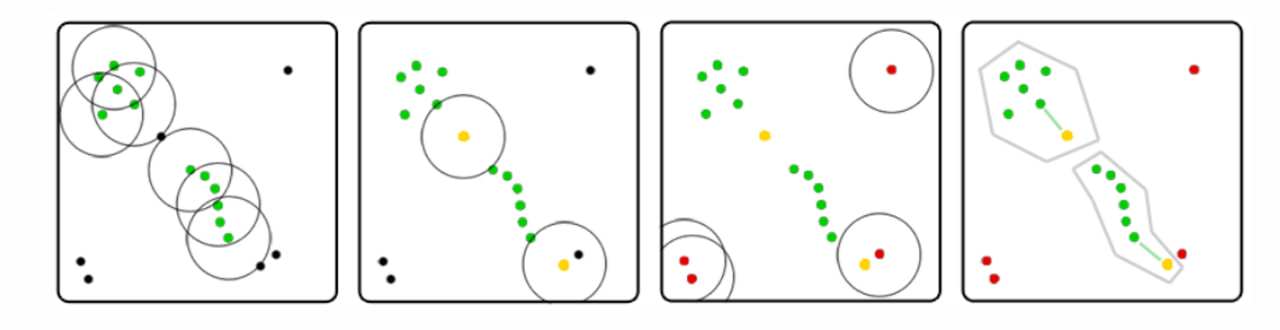
\includegraphics[width=0.85\textwidth]{dbscan_alg.jpg} 
    \end{figure}
                 
\end{frame}

\begin{frame}{DBSCAN. Алгоритм}
\textbf{Вход:} выборка $\pmb X^{n} = \{\pmb x_1, \dots, \pmb x_{n}\}$, параметры $\varepsilon$ и $m$;
	
\textbf{Выход:} разбиение выборки на кластеры и шумовые выбросы;
\begin{enumerate}
		\item $U=\pmb X^n$ --- мн-во еще не обработанных объектов, $a=0$; 
		\item \textbf{Пока} есть некластеризованные точки, т.е. $U \neq \varnothing$; 
		\item \quad взять случайную точку $\pmb x \in U$; 
		\item \quad \textbf{если} $|U_\varepsilon (\pmb x)| < m$, \textbf{то} 
		\item \quad \quad пометить $\pmb x$ как шумовой; 
		\item \quad \textbf{иначе} 
		\item \quad \quad создать новый кластер: $K=U_\varepsilon (\pmb x)$; $a = a + 1$; 
		\item \quad \quad \textbf{для всех} $\pmb x' \in K$ 
		\item \quad \quad \quad \textbf{если} $|U_\varepsilon (\pmb x')| \geq m$ \textbf{то} $K=K \cup U_\varepsilon(\pmb x')$; 
		\item \quad \quad \quad \textbf{иначе} пометить $\pmb x'$ как граничный элемент $K$; 
		\item \quad \quad соотнести объект классу $a$ для всех $\pmb x' \in K$; 
		\item \quad \quad $U=U \setminus K$ 
\end{enumerate}

\end{frame}



\begin{frame}{DBSCAN. Подбор параметров}
\small
    \begin{itemize}
        \item Значение параметра $m$ предлагается выбирать как $m\geqslant p+1$, где $p$ --- количество признаков (размерность данных). Также встречается $m=2\cdot p$.
        \item Чтобы подобрать $\varepsilon$, используют следующий алгоритм:
        \footnotesize
        \begin{itemize}
             \item[\ding{87}]  Строится график, где по оси y для каждой точки будет среднее расстояние по $m$ ближайшим соседям, а по оси~x~---~точки, отсортированные в порядке возрастания этого расстояния. 
            \item[\ding{87}]  Следует взять $\varepsilon$ где-нибудь в полосе, где происходит самый сильный перегиб. 
        \end{itemize}
    \end{itemize}
\vspace{-2.5ex}

     \begin{figure}[h]
        \centering
        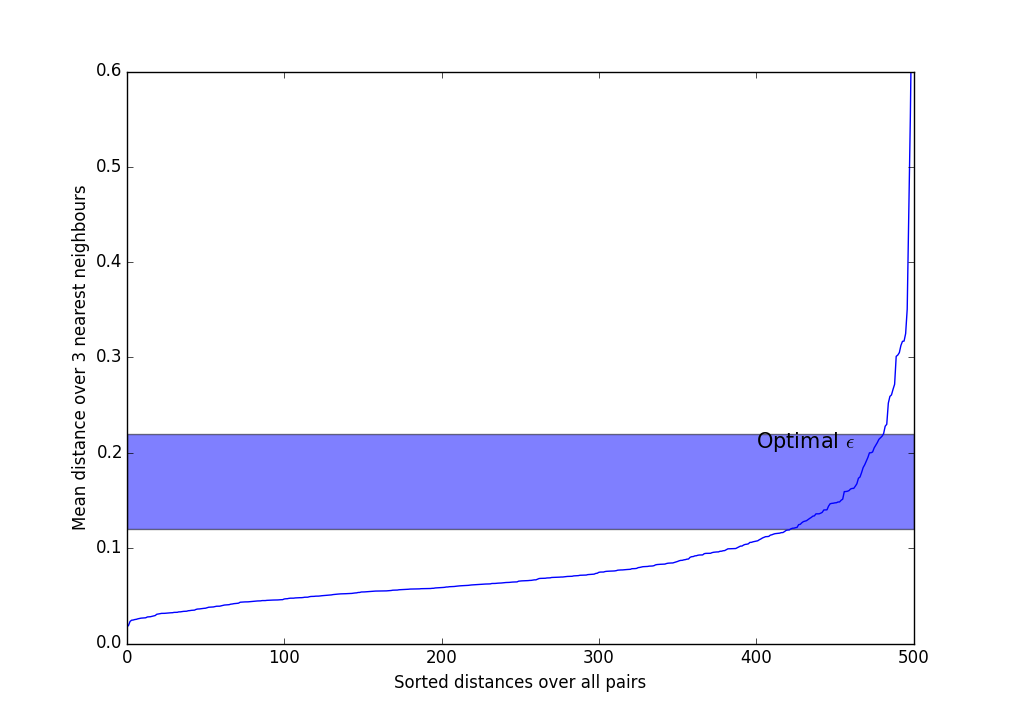
\includegraphics[width=0.45\textwidth]{dbscan_eps.png} 
    \end{figure}
                  
\end{frame}

\begin{frame}{DBSCAN. Плюсы и минусы}
    \textbf{Преимущества}:
\begin{itemize}
    \item Относительно быстро работает на больших данных;
    
    \item Устойчив к выбросам;
    
    \item Не требуется заранее указывать количество кластеров;
    
    \item Способен находить кластеры произвольной формы, а также шумовые точки в данных;

    \item Хорошо поддаётся модифицированию.
    
\end{itemize}
\vspace{1ex}

\textbf{Недостатки}:
\begin{itemize}
    \item Чувствителен к выбору параметров $\varepsilon$ и $m$;
    \item Проблемы с высокоразмерными данными (проклятие размерности);
    \item Плохо работает с кластерами разной плотности.  Не способен соединять кластеры через проёмы, и, наоборот, способен связывать явно различные кластеры через плотно населённые перемычки. 
\end{itemize}
\end{frame}

\begin{frame}{OPTICS}
  \textbf{OPTICS} (Ordering points to identify the clustering structure) ---  модификация DBSCAN для решения его ключевой проблемы: неспособности эффективно обрабатывать данные с кластерами различной плотности.
  \vspace{1ex}

  Основная идея OPTICS заключается в линейном упорядочивании точек таким образом, чтобы пространственно близкие точки становились соседними в этом упорядочивании. Этот порядок затем можно использовать для извлечения кластеров с любыми параметрами плотности.
\end{frame}

\begin{frame}{OPTICS. Определения}

\begin{itemize}
   \item \textbf{Основное расстояние} (Core Distance) $d_{core}$ --- расстояние от точки до ее $m$-го ближайшего соседа. То есть это такое минимальное расстояние $\varepsilon' \leqslant \varepsilon$, при котором точка все еще остается корневой (основной). 
   \vspace{1ex}
   
   Если такого расстояния $\leqslant \varepsilon$ не существует, $d_{core}$ считается неопределённой.

   \item \textbf{Достижимое расстояние} (Reachability Distance) --- мера того, насколько легко точка может быть достигнута из других точек в наборе данных:
\vspace{-2.5ex}

   $$d_{reach}(\pmb{a}, \pmb{b}) = \max ( d_{core} (\pmb b), \rho(\pmb a, \pmb b)),\, \text{где}\, \rho(\pmb a, \pmb b) = \text{dist}(\pmb a, \pmb b). $$    

   % Если точка находится в плотной области, то оно равно основному расстоянию. Если нет, то оно равно расстоянию до ближайшего соседа.  

   \item    Как основное, так и достижимое расстояния не определены, если нет достаточно плотного кластера (применительно к $\varepsilon$). 
\end{itemize}
\end{frame}

\begin{frame}{OPTICS. Алгоритм}
\small 
Алгоритм строит упорядочивание точек $\pi = (\pmb{x}_1, \dots, \pmb{x}_n)$ такое, что последовательность достижимых расстояний $r_i = d_{reach} (\pmb{x}_{i-1}, \, \pmb{x}_i)$ отражает переходы между плотными областями данных.

\begin{enumerate}
    \item $d_{reach} (\pmb{x} )=\infty,\quad \forall \,\pmb{x} \in \pmb{X}^n.$
    \item Для каждой непосещённой точки $\pmb{x} \in \pmb{X}^n$: 
       \begin{itemize}
           \item Вычислить $d_{core}(\pmb{x})$. 
           
           \item  Добавить $\pmb{x}$ в упорядочение $\pi$. 
           
           \item  Если $d_{core}(\pmb{x})$ определена, то для всех $\pmb{y} \in U_\varepsilon (\pmb{x})$, которые ещё не включены в упорядочение, пересчитывается их достижимость:
           \vspace{-1.5ex}
           
           $$d_{reach}(\pmb{y}) = \min (d_{reach}(\pmb{y}) , \max (d_{core}(\pmb{x}), \rho(\pmb{x}, \pmb{y})).$$
           \vspace{-1ex}

           \item Следующей выбирается точка 
           $$ p' = \arg\min_{\pmb{y} \notin \pi} d_{reach}(\pmb{y}) $$
            и процесс повторяется до тех пор, пока все точки не будут упорядочены.
       \end{itemize}
\end{enumerate}
\end{frame}

\begin{frame}{OPTICS. Извлечение кластеров}
\scriptsize
\begin{itemize}
    \item Результатом работы алгоритма является \textbf{график достижимости} --- двумерный график, где по оси x откладываются точки в порядке их обработки алгоритмом, а по оси y --- достижимое расстояние. 

    \item Поскольку точки, принадлежащие кластеру, имеют небольшое достижимое расстояние до ближайшего соседа, \textbf{кластеры} выглядят как \textbf{долины} на графике достижимости. Чем глубже долина, тем плотнее кластер.
    
    \item \textbf{Пики} на графике представляют расстояния между кластерами или переходы от кластера к шуму.
\end{itemize}

         \begin{figure}[h]
        \centering
        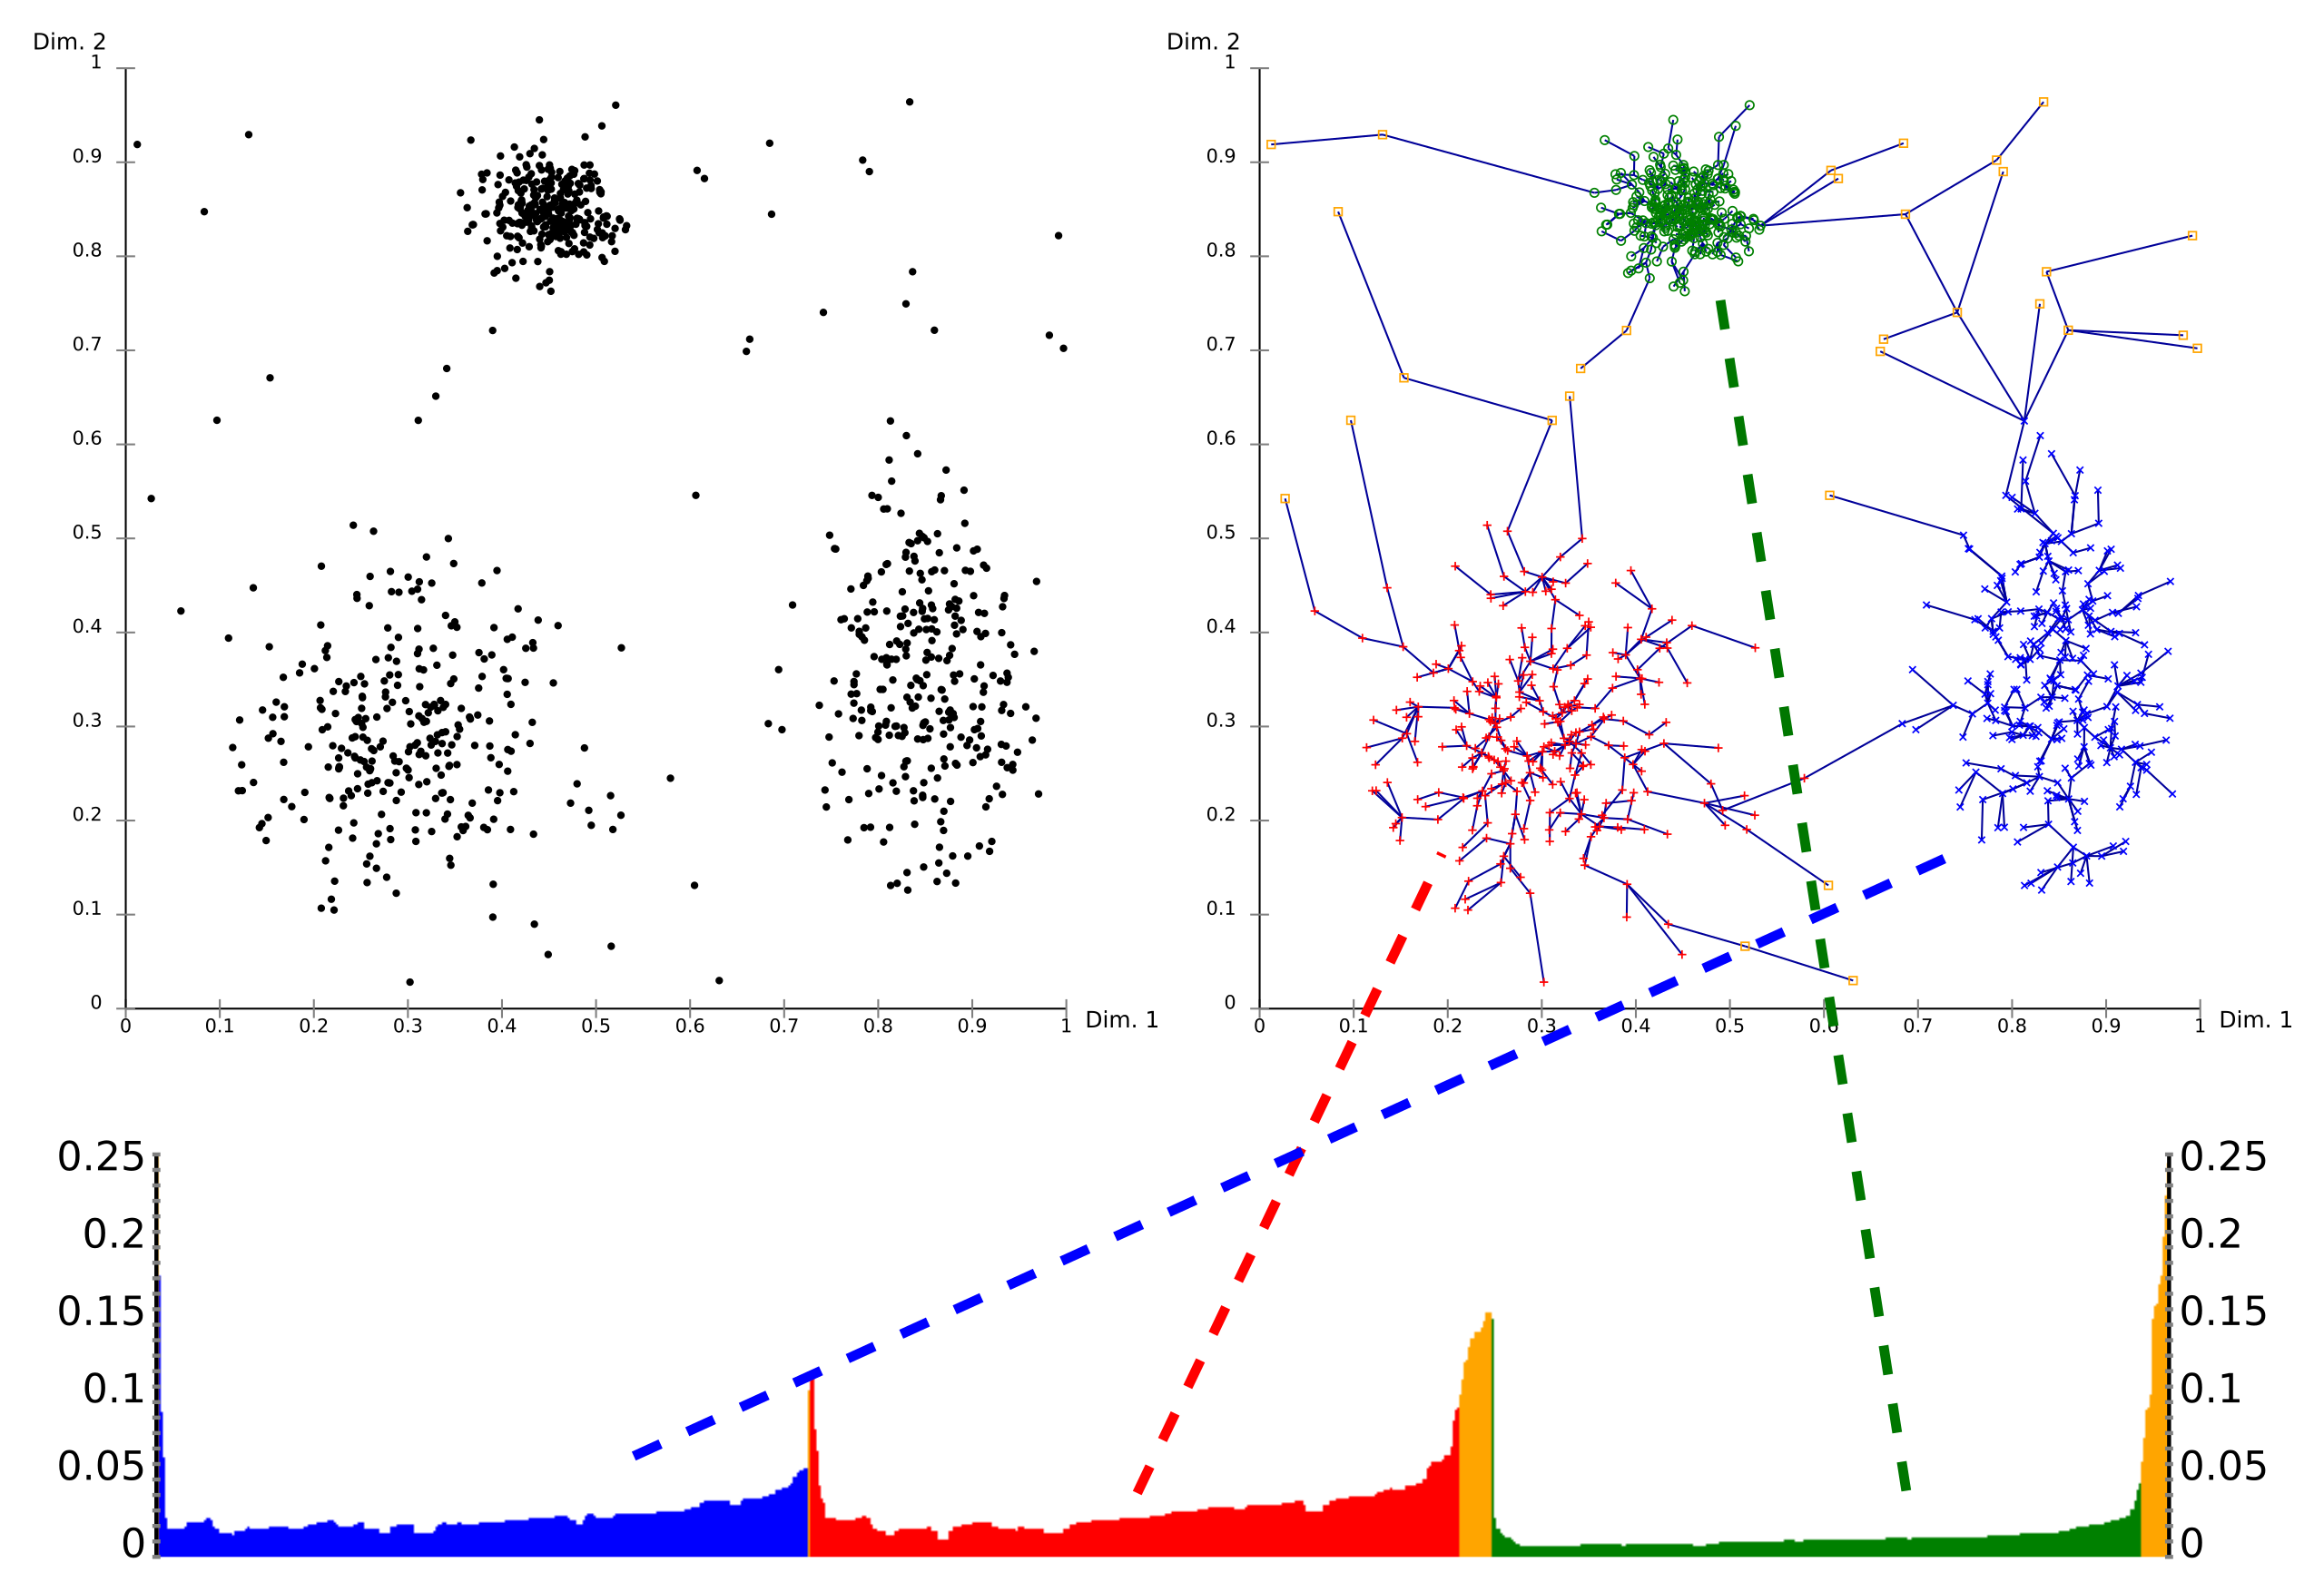
\includegraphics[width=0.6\textwidth]{optics.png} 
    \end{figure}
\end{frame}

\begin{frame}{HDBSCAN}
    \textbf{HDBSCAN} (Hierarchical DBSCAN) --- модификации DBSCAN, которая автоматически находит подходящее значение $\varepsilon$ для каждого кластера, используя иерархический подход, что позволяет определять кластеры с разной плотностью.
    \vspace{1ex}
    
    По сравнению с DBSCAN  для него требуется большее количество вычислений, что увеличивает время работы алгоритма.
\end{frame}


\begin{frame}{HDBSCAN. Определения}
\small 
\begin{itemize}
    \item \textbf{Основное расстояние} (Core Distance) $d_{core}$ --- расстояние от точки до ее $m$-го ближайшего соседа. Это величина, показывающая, насколько плотна область вокруг точки.
\vspace{1ex}

    \item \textbf{Взаимное достижимое расстояние} (Mutual Reachability Distance) --- специальная метрика:
$$d_{mreach}(\pmb{a}, \pmb{b}) = \max (d_{core}(\pmb a), d_{core} (\pmb b), \rho(\pmb a, \pmb b)),\, \text{где}\, \rho(\pmb a, \pmb b) = \text{dist}(\pmb a, \pmb b). $$
\vspace{-2ex}

 Расстояния между точками в областях высокой плотности (с малым $d_{core}$) остаются неизменными, а расстояния между точками в областях низкой плотности (с большим $d_{core}$) увеличиваются. Таким образом, общий эффект использования MRD в качестве метрики расстояния заключается в том, что точки в областях с низкой плотностью отдаляются от точек в областях с высокой плотностью.
\vspace{0.5ex}

Это делает алгоритм устойчивым к разной плотности.
\end{itemize}
\end{frame}

\begin{frame}{HDBSCAN. Алгоритм}
    \begin{enumerate}
        \item Для каждой точки рассчитывается $d_{core}$.
        
        \item  Вычисляем MRD между всеми парами точек, строим полный взвешенный граф.

        \item На графе взаимной достижимости строим минимальное остовное дерево (MST).

        \item Строим иерархию кластеров (преобразовываем MST в дендрограмму):
        % \begin{itemize}
        %     \item  Сортируем рёбра MST по весу в порядке убывания;
        %     \item Последовательно удаляем рёбра, начиная с самого тяжелого (т.е. с наименее плотной связью);
        %     \item Каждое удаление ребра разделяет дерево на компоненты связности.
        % \end{itemize}

        % Этот шаг эквивалентен  применению разрезов к дендрограмме, полученной с помощью иерархической кластеризации с правилом слияния single linkage и метрикой определяемой расстоянием взаимной достижимости.
        \begin{itemize}
            \item Сортируем рёбра MST по весу в порядке возрастания;
            \item Начиная с самого маленького расстояния, рёбра последовательно добавляются, соединяя точки и формируя кластеры.
        \end{itemize}
    \end{enumerate}
\end{frame}

\begin{frame}{HDBSCAN. Алгоритм}
\footnotesize
\begin{enumerate}
   \setcounter{enumi}{4}
    \item Введём параметр $\hat m$ --- минимальное число точек в кластере и новую шкалу для дендрограммы $\lambda = 1/d_{mreach}$.
    
    \item Будем рассматривать дендрограмму снизу вверх по мере убывания $\lambda$ (возрастания $d_{mreach}$). Мы скажем, что множество узлов $C_i$, получающееся рассмотрением связного поддерева в дендрограмме на высоте $\lambda$, является кластером, если оно содержит хотя бы $\hat m$ вершин. Максимальное такое $\lambda$ назовем $\lambda_{i, \text{death}}$.
    
    \item Минимальную величину $\lambda$, на которой поддерево $C_t$ распадается на два кластера $C_i$ и $C_j$, назовём $\lambda_{i, \text{birth}} = \lambda_{j, \text{birth}} = \lambda_{t, \text{death}}$.
    
    \item Разбиваем точки на кластеры так, чтобы 
    $$\max \sum_{i \in \mathcal{C}} \int_{\lambda_{i, \text{birth}}}^{\lambda_{i, \text{death}}} p_{i, \lambda} d \lambda,$$ 
    
    где $p_{i, \lambda}$ --- это число точек в кластере $C_i$ на уровне $\lambda$.
    
    \item Не попавшие в разбиение точки объявляем выбросами.
\end{enumerate}
\end{frame}

\begin{frame}{HDBSCAN. Иллюстрация}
     \begin{figure}[h]
        \centering
        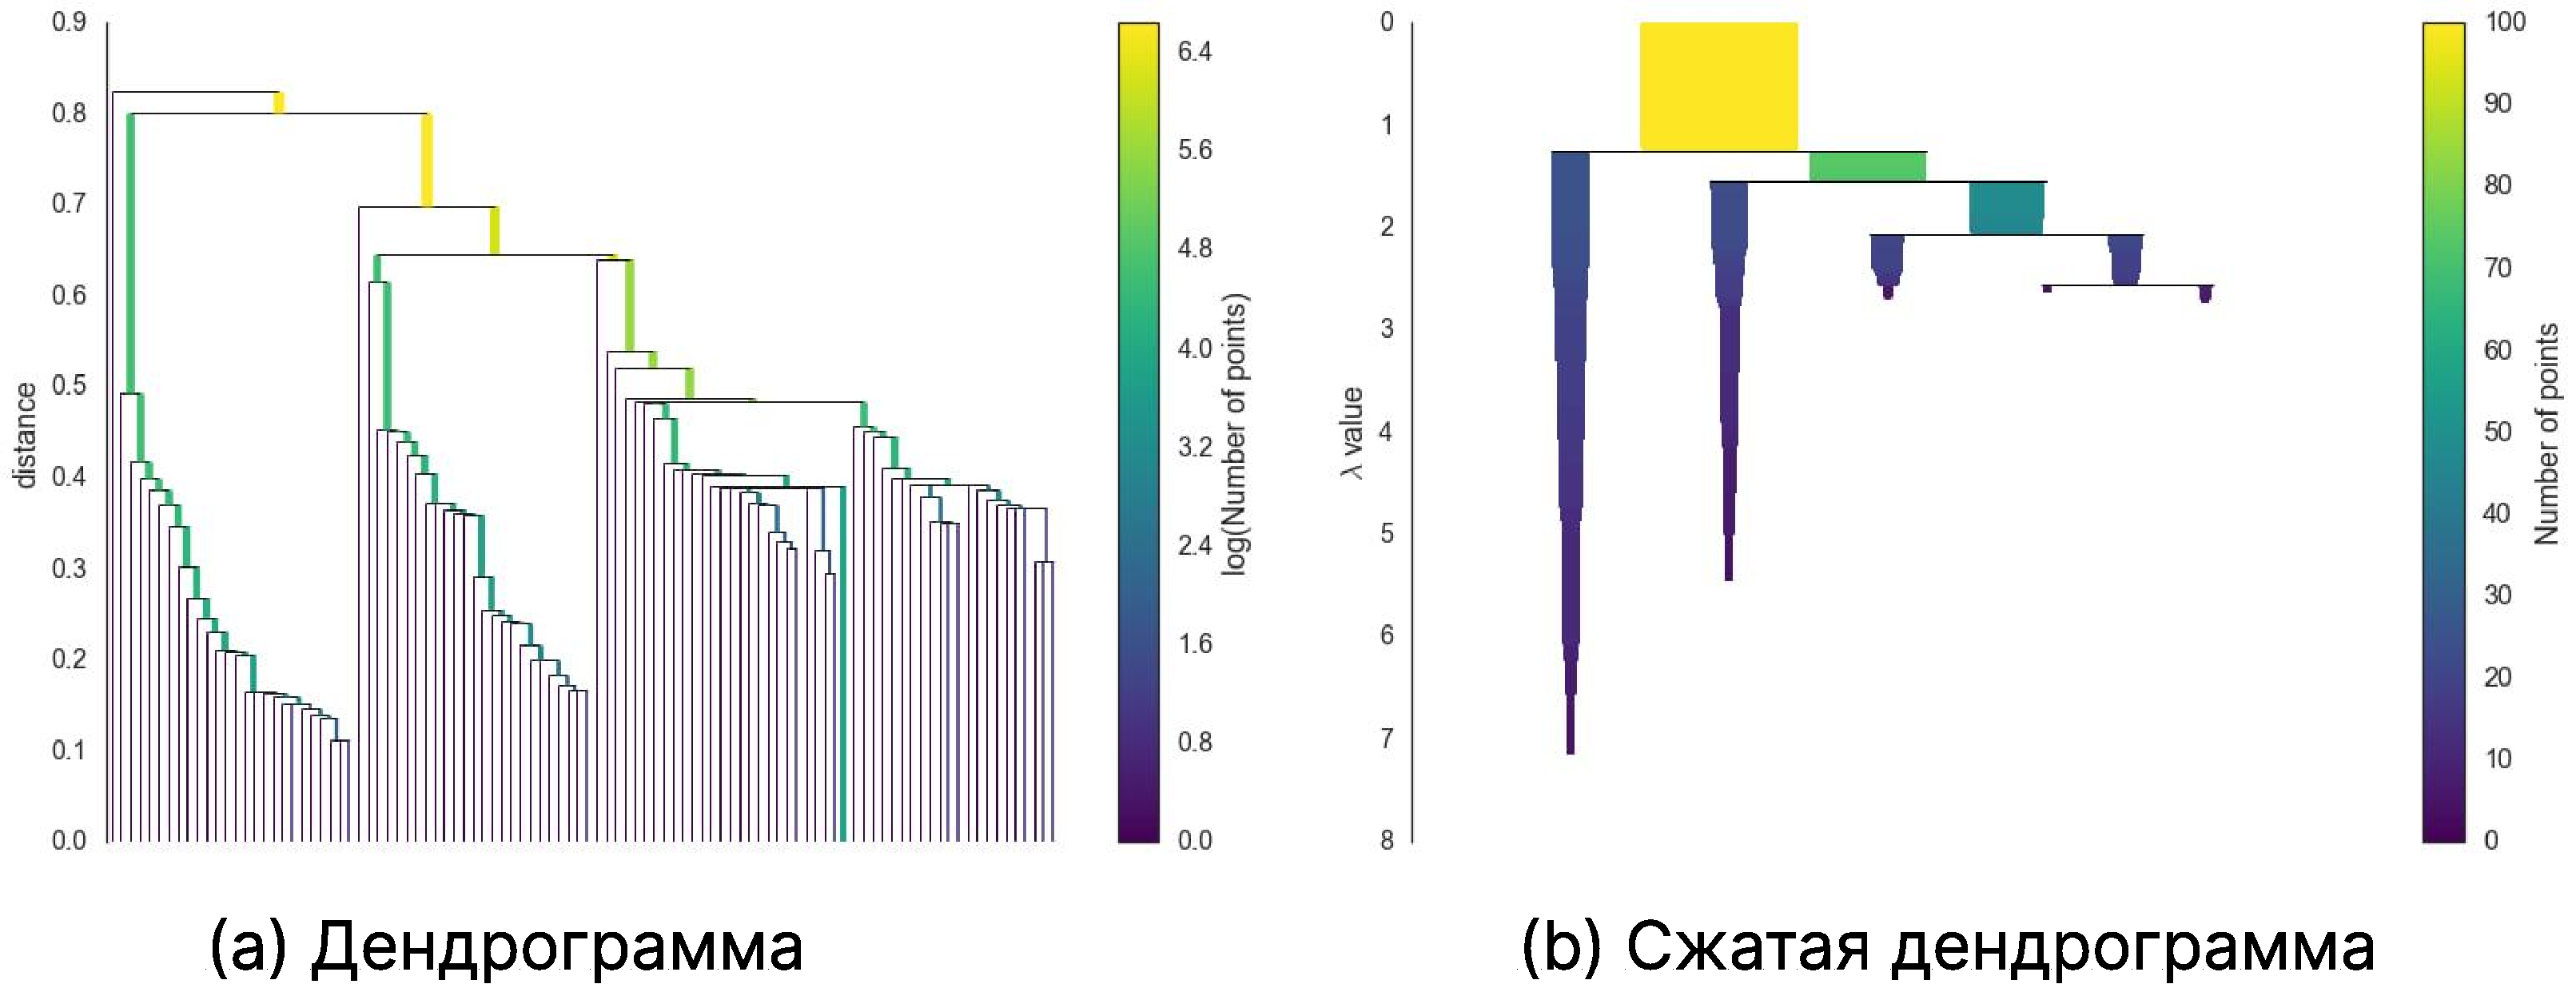
\includegraphics[width=1.01\textwidth]{hdbscan.pdf} 
    \end{figure}
\end{frame}

\begin{frame}{CLIQUE}
\small 

    \textbf{CLIQUE} (CLustering In QUEst) --- это алгоритм, который комбинирует в себе идеи сеточного подхода к кластеризации и подхода, основанного на подпространствах, для обнаружения плотных кластеров в подпространствах максимальной размерности.
\vspace{1.2ex}

    \emph{Мотивация}: В данных с большим количеством признаков <<проклятие размерности>> приводит к тому, что данные становятся очень разреженными. Кластеры часто существуют только в пределах небольшого подмножества признаков, а в других измерениях точки могут быть распределены случайным образом. CLIQUE создан для решения именно этой проблемы.
\end{frame}

\begin{frame}{CLIQUE. Определения}
\small 

У алгоритма два входных параметра:
 \begin{itemize}
    \item[\ding{87}] $\xi$ --- параметр сетки;
    \item[\ding{87}] $\tau$ --- пороговое значение плотности.
\end{itemize}
\vspace{1ex}


\begin{itemize}
    \item Пространство признаков разбивается на $\xi$ равных частей по каждому признаку. Пересечение одного интервала из каждого измерения называется \textbf{единицей} (unit).

    \item \textbf{Селективность} (selectivity) единицы определяется как доля общего количества точек данных, содержащихся в этой единице. 

    \item \textbf{Плотная единица} (dense unit) --- единица считается плотной, если ее селективность превышает пороговое значение плотности~$\tau$.

    \item \textbf{Кластер} --- максимальное множество связанных (т.е. имеющих общую грань) плотных единиц в одном и том же подпространстве.
\end{itemize}

\end{frame}

\begin{frame}{CLIQUE. Описание кластеров}
\small

\begin{itemize}
%\item \textbf{Область} (region) в $k$ измерениях ---  это прямоугольное $k$-мерное множество, сонаправленное осям. Мы интересуемся только теми областями, которые могут быть выражены как объединения единиц.

%\item Область может быть выражена в \textbf{дизъюнктивной нормальной форме} (ДНФ).

    \item CLIQUE генерирует описания кластеров в виде выражений в \textbf{дизъюнктивной нормальной форме} (ДНФ), покрывая кластер минимальным количеством максимальных, возможно перекрывающихся, прямоугольников и описывая кластер как объединение этих прямоугольников. 

   % \item Каждая единица в $k$-мерном подпространстве может быть описана как конъюнкция неравенств, потому что она представляет собой пересечение $2k$ полупространств, параллельных осям и определенных $k$ одномерными интервалами. Поскольку каждый кластер состоит из объединения этих ячеек, его представление может быть выражено через ДНФ. 


    %\item Этот подход позволяет получить компактное и минимальное описание кластеров, что облегчает пользователям понимание результатов.

    \item Кроме того, последний шаг CLIQUE принимает в качестве входных данных покрытие для каждого кластера и находит минимальное покрытие, определяемое с точки зрения количества максимальных областей (прямоугольников), необходимых для покрытия кластера.
\end{itemize}
\end{frame}

\begin{frame}{CLIQUE. Иллюстрация определений}

     \begin{figure}[h]
        \centering
        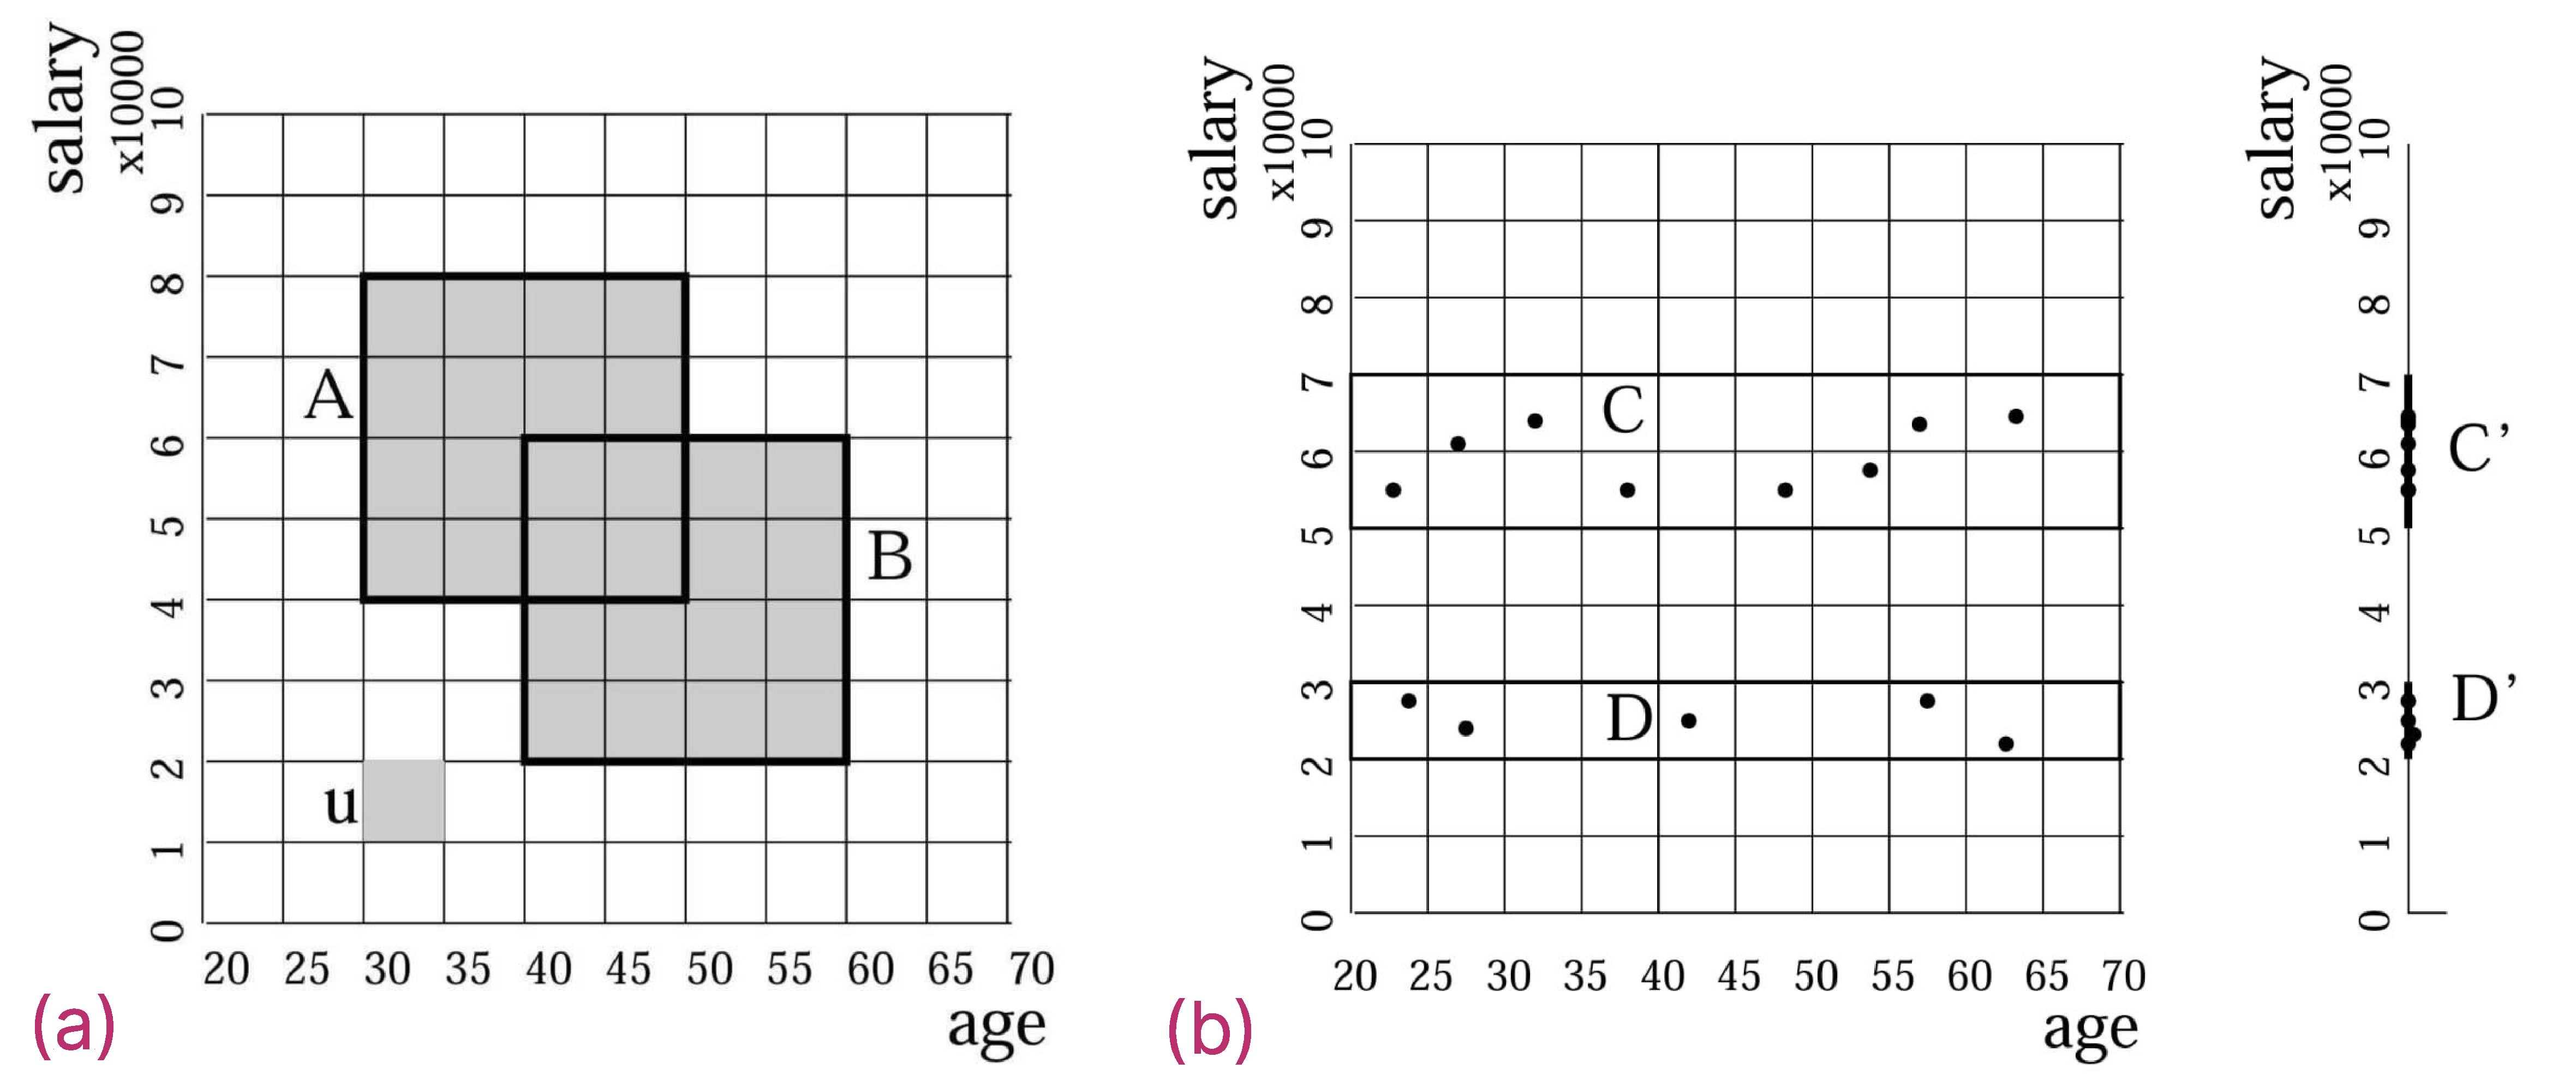
\includegraphics[width=0.8\textwidth]{clique.pdf} 
    \end{figure}
\vspace{-2ex}

\footnotesize
\begin{itemize}
    \item[\ding{87}] График (a): сетка $10\times 10$, единица --- $u$, кластер $A\cup B$, его мин. описание в виде ДНФ 
    \begin{footnotesize}
    $$ ((30 \leq \text{age}  < 50) \land (4 \leq  \text{salary} < 8)) \vee ((40 \leq  \text{age}  < 60) \land (2 \leq  \text{salary} < 6)).$$
    \end{footnotesize}
    \item[\ding{87}] График (b): $\tau=20\%$ , ни одна двумерная единица не является плотной, и в исходном пространстве данных нет кластеров.   Однако если спроецировать точки на измерение зарплаты, то получим три одномерные плотные единицы. Две из них соединены, поэтому в одномерном подпространстве зарплаты есть два кластера.
\end{itemize}

\end{frame}

\begin{frame}{CLIQUE. 3 основных этапа}
\footnotesize
    \begin{enumerate}
        \item \textbf{Поиск плотных подпространств}
        \begin{itemize}
         \scriptsize
            \item Представляем данные как $\xi$-мерную сетку;
            
            \item Находим \textbf{плотные ячейки} (где точек > порога $\tau$);
            
            \item Поиск плотных единиц в подпр-ах высокой размерности ведется снизу вверх, начиная с 1-мерных подпр-в. Используем принцип \textbf{монотонности}: <<Если k-мерная ячейка плотная, то все её (k-1)-мерные проекции тоже плотные>>.
        \end{itemize}
        
        \item \textbf{Формирование кластеров}
        \begin{itemize}
           \scriptsize
            \item После того как найдены все плотные k-мерные единицы в определенном подпространстве, алгоритм объединяет их в кластеры;
            
            \item Строится граф , где вершины --- это плотные единицы, а ребра соединяют соседние единицы;
            
            \item Все связанные плотные единицы объединяются в один кластер. Для этого используется алгоритм поиска в глубину (DFS).
        \end{itemize}
        
        \item \textbf{Генерация описаний}
        \begin{itemize}
            \scriptsize
            \item Покрываем кластер \textbf{минимальным количеством максимальных прямоугольников};

            \item Строим \textbf{минимальное покрытие}: удаляются те прямоугольники, которые полностью покрываются другими, более крупными прямоугольниками из покрытия;
            
            \item Записываем результат в виде \textbf{ДНФ-формул}.
        \end{itemize}
    \end{enumerate}
\end{frame}


\begin{frame}{CLIQUE. Плюсы и минусы}
    \textbf{Преимущества}:
\begin{itemize}
    \item Хорошо работает для данных с большой размерностью;
    
    \item Не требует знания числа кластеров заранее, они формируются автоматически из плотных ячеек;
    
    \item Каждый кластер можно описать в логической форме;

    \item  Алгоритм устойчив к пропущенным значениям во входных данных.
    
\end{itemize}
\vspace{1ex}

\textbf{Недостатки}:
\begin{itemize}
    \item Результат сильно зависит от входных параметров: размера сетки и пороговой плотности;
    \item Размер сетки растёт экспоненциально с размерностью.
\end{itemize}
\end{frame}


\begin{frame}{Сравнение методов}
         \begin{figure}[h]
        \centering
        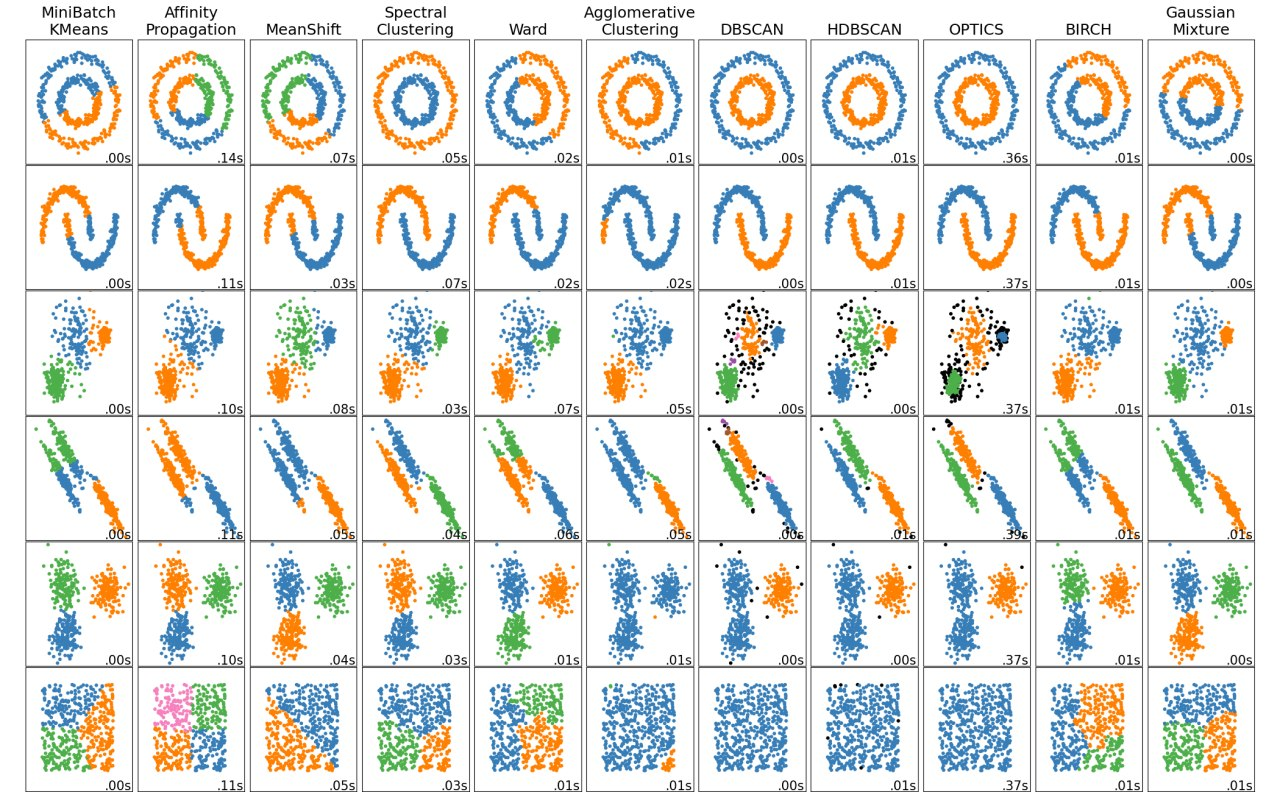
\includegraphics[width=1\textwidth]{clast_comp.jpg} 
    \end{figure}
\end{frame}

\begin{frame}{Функционалы качества кластеризации}
\small
Задачу кластеризации можно ставить как задачу \emph{дискретной оптимизации}: необходимо так приписать номера кластеров $y_i$ объектам $\pmb{x}_i$, чтобы значение выбранного функционала качества приняло наилучшее значение. 
 
    \begin{itemize}

 \item  \textbf{Среднее внутрикластерное расстояние}: $$F_0 = \frac{\sum_{i < j}\mathbf{I}_{\{y_i = y_j\}}\rho(\pmb{x}_i, \pmb{x}_j)}{\sum_{i < j}\mathbf{I}_{\{y_i = y_j\}}}\to \min .$$
       \item \textbf{Среднее межкластерное расстояние}: $$F_1 = \frac{\sum_{i < j}\mathbf{I}_{\{y_i \neq y_j\}}\rho(\pmb{x}_i,\pmb{x}_j)}{\sum_{i < j}\mathbf{I}_{\{y_i \neq y_j\}}}\to \max.$$
   \end{itemize}
   
На практике вычисляют отношение пары функционалов, чтобы учесть как межкластерные, так и внутрикластерные расстояния: $$F_0/F_1\to\min$$.
\end{frame}


\begin{frame}{Функционалы качества кластеризации. Silhouette}
\footnotesize

\begin{itemize}
\item Пусть \( a \) и \( b \) есть среднее расстояние между наблюдением и всеми другими точками в том же кластере/в следующем ближайшем кластере
\item Коэффициент силуэта для наблюдения есть
\[s = \frac{b - a}{\max(a, b)}\]
\item Для выборки коэффициент силуэта задается средним значением коэффициентов каждого наблюдения
\item Значения в интервале [-1; 1]. Чем больше, тем лучше. Если коэффициент близок к 0, то это свидетельство в сторону того, что кластеры "накладываются" друг на друга
\end{itemize}

\end{frame}

\begin{frame}{Функционалы качества кластеризации. Calinski-Harabasz Index (Variance Ratio Criterion)}
\footnotesize

\begin{itemize}
\item Индекс Калинского–Харабэсза определяется как отношение между средней межкластерной дисперсией и средней дисперсией внутри кластеров
\[s = \frac{\operatorname{tr}(B)}{k - 1} / \frac{\operatorname{tr}(W)}{n - k}\]
\item Тут \( k \) – число кластеров, а матрицы \( B \) и \( W \) имеют вид
\[W = \sum_{q=1}^{k} \sum_{x \in C_q} (x - c_q)(x - c_q)^T, \quad B = \sum_{q=1}^{k} n_q(c_q - c_x)(c_q - c_E)^T\]
где \( C_q \) – наблюдения из кластера \( q \), \( c_q \) – центр кластера \( q \), \( c_x \) – центр всего набора данных \( X \), а \( n_q \) – число наблюдений в кластере \( q \).
\item Значение индекса тем больше, чем разделеннее кластеры и чем более сгруппированы в кластерах наблюдения. Ну и применять для случая сферических/эллиптических кластеров
\end{itemize}

\end{frame}

\begin{frame}{Функционалы качества кластеризации. Davies-Bouldin Index}
\footnotesize

\begin{itemize}
\item Индекс Дэвиса–Болдина оценивает среднее "сходство" между кластерами, где сходство есть мера, которая сравнивает расстояние между кластерами с размером самих кластеров
\item Пусть \( s_i \) есть среднее расстояние между каждой точкой кластера \( i \) и центроидом этого кластера, а \( d_{ij} \) есть расстояние между центроидами кластеров. Определим схожесть между кластерами следующим образом
\[R_{ij} = \frac{s_i + s_j}{d_{ij}}\]
\item Тогда индекс имеет вид
\[DB = \frac{1}{k} \sum_{i=1}^{k} \max_{i\neq j} R_{ij}\]
\item Чем индекс меньше, тем лучше. Близок к 0 – отличное разделение. Недостаток тот же, что и у индекса Калинского–Харабэсза
\end{itemize}

\end{frame}


\end{document}
